
\chapter{Designing a Synchronization Framework}\label{main}

\section{Application Scenarios}
We describe common synchronization scenarios based on popular mobile applications.

\subsection{A Collaborative Task Manager}

The seemingly simple scenario of a Task Manager turns out to be very complex to implement if enhanced with collaborative features and offline availability.

Let us first look at some user stories and then try to define a suitable data model for such an application.

\subsubsection{User Story 1: Creating Projects}
\begin{itemize}
\item A User can create Projects in order to coordinate Tasks.
\item A User can invite other Users as Project Members to a Project.
\end{itemize}

Examples for Projects created by User Rita would be:\\

\begin{tabular}{ l l }
Project Name & Members \\
\hline
Marketing Material & Rita, Tom, Allen \\
Product Roadmap & Rita, Allen \\
Sales Review & Rita, Lisa
\end{tabular}

\subsubsection{User Story 2: Creating and Editing Tasks}
\begin{itemize}
\item Project Members can add Tasks to a Project in order to manage responsibilities.
\item A Task can have a due date and responsible project member assigned.
\item A Task can be edited by Project Members and marked as done.
\item A Task can be moved in the list of Tasks.
\end{itemize}

An example list of Tasks could be:\\

\begin{tabular}{ l l l l }
\multicolumn{4}{ c }{Project "Marketing Material"} \\
Task & Due Date & Assignee & Done \\
\hline
Create event poster & 2013-08-12 & Rita & No\\
Write blog entry on event & 2013-07-20 & Tom & Yes
\end{tabular}

\subsubsection{User Story 3: Commenting on Tasks}
\begin{itemize}
\item Project Members can add Comments to Tasks
\end{itemize}

Examples would be:\\

\begin{tabular}{ l l l }
\multicolumn{3}{ c }{Task "Create event poster" in Project "Marketing Material"} \\
Member & Date & Comment \\
\hline
Rita & 2013-07-20 & Allen, I need you to create some graphics. \\
Allen & 2014-07-20 & Ok, lets go through it tomorrow morning!
\end{tabular}

\subsubsection{User Story 3: User Workflows}
\begin{itemize}
\item In order to be productive a user needs to access all Tasks from any device.
\item A user should be able to Edit and Create Projects and Tasks when disconnected from any network.
\item The data should be kept as current as possible even if a user's device does not have reliable internet access.
\end{itemize}

An example workflow that should be supported:\\

\begin{itemize}
\item Rita works at the desktop computer in her office with high-speed internet access. She creates Project A and invites Allen.
\item Allen works from home on his notebook with high-speed internet access. He reviews the Project and creates task A1.
\item Rita is already on her way home but has mobile internet access on her smartphone. She receives the added task A1 and edits its title.
\item Rita is still on the train but decides to continue working on her notebook. Her notebook does not have internet access but she can establish a direct connection to her smartphone via Wifi. The reception on her smartphone has dropped in the meanwhile. She receives the latest updates from her smartphone and adds a comment to task A1.
\item Allen who is still at home can not receive Rita's comment as she is still on the train. In the meanwhile he creates a Task A2 in Project A.
\item Rite gets home where she has internet access with her notebook. She receives Allen's created Task A2.
\item Allen, who is still at his notebook, receives Rita's comment as soon as she connects to internet at home.
\end{itemize}

\subsubsection{Data Model}
Based on the user stories we can derive a plausible data model for the application. We can map it to a straight-forward entity-relationship model as shown in figure \ref{fig:tasks-data-model}.\\
The only complication is the requirement of Tasks per Project being ordered. We model this as a linked list by having a "Next Task" relationship.

\begin{figure}[tasks-data-model]
\centering
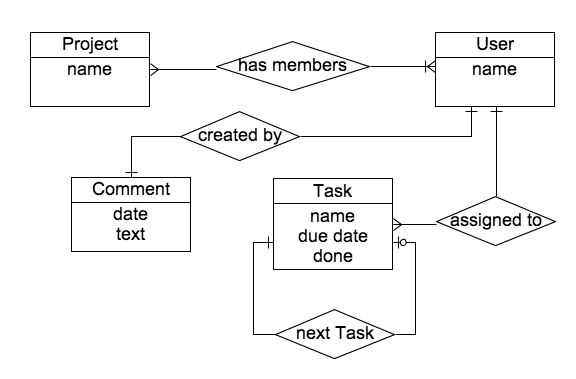
\includegraphics[width=0.8\textwidth]{img/tasks-schema}
\caption{A collaborative Task Manager's data model}
\label{fig:tasks-data-model}
\end{figure}

\subsection{A File Sharing App}

Dropbox synchronizes a file system - it is therefore a good example for
syncing of hierarchical data.

The data model is simple:

\begin{itemize}
\item Tree Item (name)
\item Tree extends Tree Item (has children of type Tree Items)
\item Data extends Tree Item (data)
\end{itemize}

The list of child Tree Items can either be ordered or unordered. While
Dropbox does not sync the order of files there are scenarios where this
is required.

Syncing trees can trigger conflicts if sub trees have been modified
concurrently.

\subsection{(Text Synchronization)}

Collaborative document editors like Google Docs need to synchronize text
that is concurrently edited.\\Google Docs currently does not support
offline editing.

Syncing text is equal to the problem of syncing an ordered list and can
trigger conflicts.

\section{Requirements}
\label{sec:requirements}
From the common scenarios we derive a set of requirements for a synchronization solution.

Requirements for strategies:

\begin{itemize}
\item Causality preservation
\item Eventual consistency
\item Optimistic synchronization
\item Expose conflicts
\item Support peer-to-peer or hybrid synchronization
\item Integration with existing app logic
\end{itemize}

(TODO: need to explain why this set of requirements, constraints on
mobile devices\ldots{})

Aspects to consider when evaluating strategies:

\begin{itemize}
\item How are updates detected?
\item How are updates propagated? (Stream or Snapshot)
\item How are updates merged/reconciled? (State or Edit-based)
\item Level of structural awareness (Textual, Syntactic, Semantic/Structural)
\end{itemize}

\section{Evaluating Existing Systems}
Here we evaluate existing solutions based on the requirements.

\subsection{git}

\begin{itemize}
\item
  Data structure: filesystem/tree
\item
  Merging: tree-based, three-way merge
\item
  Propagation: snapshot-based
\item
  Supports peer-to-peer
\end{itemize}

\subsection{CouchDB}

\begin{itemize}
\item
  Data structure: key-value
\item
  Merging: tree-based
\item
  Propagation: stream-based
\item
  Supports peer-to-peer
\end{itemize}

\subsection{(Backends-as-a-Service)}
- parse.com
- stackmob
- deployd

Most of them simply expose a REST-API but leave all the conflict handling work to the app developer.\\
Are completely centralized.

\section{Architecture of Synclib}
Based on the requirements and the evaluation of existing systems we derive a unique architecture for a practical synchronization solution.

\begin{itemize}
\item
  \textbf{no timestamps}: state-based 3-way merging
\item
  \textbf{no change tracing}: change tracing is not necessary - support
  diff computation on the fly
\item
  \textbf{data agnostic}: leave diff and merge of the actual data to
  plugins
\item
  \textbf{distributed}: syncing does not require a central server
\item
  \textbf{be small}: only implement the functional parts of syncing -
  leave everything else to the application (transport, persistence)
\item
  \textbf{sensitive defaults}: have defaults that \emph{just work} but
  still support custom logic (e.g.~for conflict resolution)
\end{itemize}

- cross-platform through web standards
- solve server behaviour through native proxy
- diff-merge-patch
- most-recent-common-ancestor

\section{Technologies used for Implementation}
We describe implementation details like the technologies used, code structure and the testing framework to evaluate the system.

- everything web-based --> only way to be cross-platform
- client-side persistence with HTML5
- note on alternatives (Lua, native)

\section{Differencing and Merging of Data Models}
- explain diff, merge and patch
- implement diff, merge and patch logic for primitive data structures
  -> use them to recursively model complex data structures
- ensure conflicts are made explicit

\subsection{Sets}
\subsection{Ordered Lists}
\subsection{Ordered Sets}
\subsection{Dictionaries}
used for object collections in data models
\subsection{Ordered Dictionaries}
most common for managing ordered object collections in data models
can be modeled with dictionary and ordered set/list
\subsection{Trees}
- tree as an example for composite data model
- efficient child tree pointers like in git

\subsection{Composite Data Structures}
- show how to represent complex data models as composite data structures

\section{Storing and Commiting Changes}
As syncing is state based we need to track the history of edits on each client.\\Each client has his own replica of the database and commits
data locally.\\On every commit we create a commit object that links both
to the new version of the data and the previous commit.\\

- use content-adressable store
- only store changes and reference unchanged data through hashs --> like git
- commit links to data and parent commit

\section{Finding Common Commits}
- Most Recent Common Ancestor algorithm used for finding common commit of clients
- described algorithm in background
- implementation as separate module

\section{Synchronization Protocol}
If a client is connected to a server he will start the sync process on every commit. As
synclib2's architecture is distributed a server could itself be a client
who is connected to other servers.\\To the latest commit on a database
we refer to as the `head'.

Synchronization follows the following protocol:

\begin{verbatim}
Client has committed to its local database.
Client pushs all commits since the last synced commit to Server.
Client asks Server for the common ancestor of client's head and the server's head
Client pushs all changed data since the common ancestor to Server.

if common ancestor == server head
  // there is no data to merge
  try fast-forward of server's head to client's head
  if failed (someone else updated server's head in the meantime) then start over
else
  Client asks Server for all commits + data since the common ancestor
  Client does a local merge and commits it to the local database
  start over
\end{verbatim}

This protocol is able to minimize the amount of data sent between synced
stores even in a distributed, peer-to-peer setting.

Updating the server's head uses optimistic locking. To update the head
you need to include the last read head in your request.

\section{Handling Conflicts}

\section{Integration with Application Logic}
- demonstrate how to interface with standard MVC frameworks like Backbone, Ember.js

\section{(Managing Changes to Distributed Logic)}
The additional client logic has to be maintained and upgraded for new releases of the application. As the client logic is distributed among all users of the application, a code upgrade becomes more complex to manage than a simple server update. We will see how the same logic used to synchronize application data can be used for updating distributed application code.

- on the server its easy - we can use a distributed version control system
- they don't run on the client -> we need an app-embedded solution

